% !TeX root = ../main.tex

\chapter{Method}
\label{ch:method}

This chapter describes what was actually built. Section~\ref{sec:method-problem} states the distillation problem in precise terms. Section~\ref{sec:method-data} describes the Taiwan RWRF dataset and its normalisation. Section~\ref{sec:method-datasources} documents the underlying data sources and the preprocessing pipeline that turns them into the training Zarr store. Section~\ref{sec:method-teacher} recaps the frozen teacher. Sections~\ref{sec:method-pd} and \ref{sec:method-cd} describe the progressive-distillation and consistency-distillation pipelines respectively. Section~\ref{sec:method-flowcast} describes FlowCast, a Conditional Flow Matching student that bypasses the teacher ODE entirely. Section~\ref{sec:method-qpepre} describes the dataset-specific loss modifications for the precipitation channel. Section~\ref{sec:method-infra} documents the training infrastructure.

% ==================================================
\section{Problem Setup}
\label{sec:method-problem}

Let $\Dteach$ denote the frozen EDM teacher diffusion network and $\Freg$ the frozen deterministic regression network, both provided as pretrained checkpoints. Given conditioning $c_t = \mathrm{concat}(X_{t-1}, S_t, M_t, I)$, where $M_t = \Freg(X_{t-1}, S_t, I)$, the teacher samples a residual $\hat{R}_t$ by integrating the PF-ODE from $\sigma_{\max}$ to $\sigma_{\min}$ using a Heun sampler with $N_{\text{teach}} \approx 13$ steps (so $\approx 25$ NFE per hourly forecast step). The full prediction is $\hat{X}_t^{\text{teach}} = M_t + \hat{R}_t$.

The student $\Dnet$ shares the teacher's architecture (an EDMPrecond SongUNet with the same conditioning interface) and is trained so that, given the same conditioning $c_t$, it produces a sample $\hat{X}_t^{\text{stud}} \approx \hat{X}_t^{\text{teach}}$ with at most $K \in \{1, 2, 4, 8\}$ NFE. We study two training procedures: progressive distillation, which directly halves the teacher step count in stages, and consistency distillation, which trains the student to satisfy a self-consistency property along teacher trajectories.

% ==================================================
\section{Dataset: Taiwan RWRF}
\label{sec:method-data}

The training data live in a Zarr store under the project directory (see Appendix~\ref{app:repro}). The store has three top-level groups.

\paragraph{LowRes conditioning $S_t$.} Shape $(T, 24, 224, 128)$, where $T$ is the hourly time index and the 24 channels are mean sea-level pressure, two-metre temperature, ten-metre winds, and the specific humidity, temperature, and zonal and meridional winds at four pressure levels (\SIlist{1000;850;500;250}{\hecto\pascal}). These channels are low-resolution re-gridded ERA5 fields that serve as synoptic-scale boundary conditioning.

\paragraph{HighRes target $X_t$.} Shape $(T, 4, 224, 128)$, with four channels: two-metre temperature (\texttt{t2m}), ten-metre zonal and meridional winds (\texttt{u10}, \texttt{v10}), and hourly accumulated precipitation (\texttt{qpepre}). The horizontal grid covers Taiwan from \SI{21.6}{\degree} to \SI{25.6}{\degree}N and \SI{119.75}{\degree} to \SI{122.25}{\degree}E at approximately \SI{2}{\kilo\metre} resolution. The dataset splits into 21{,}216 training hours (2019-08 through 2021-12) and 8{,}760 validation hours (calendar year 2022).

\paragraph{Invariants $I$.} Shape $(2, 224, 128)$, channels land--sea mask and orography. These are broadcast across time and concatenated into the conditioning bundle.

\paragraph{Normalisation.} Per-channel means and standard deviations are computed on the training split and stored in the Zarr metadata. The HighRes statistics are
\begin{equation}
  \mu_{\text{HR}} = (295.98,\; -1.58,\; -2.65,\; 0.182), \qquad
  \sigma_{\text{HR}} = (5.61,\; 3.84,\; 5.66,\; 9.12),
  \label{eq:hr-stats}
\end{equation}
which show that \texttt{qpepre} has a near-zero mean with standard deviation an order of magnitude larger than its mean --- a direct fingerprint of its heavy-tailed, sparse distribution. Training and validation losses are computed on normalised fields; metrics in Chapter~\ref{ch:experiments} are reported on denormalised fields with physical units.

% ==================================================
\section{Data Sources and Preprocessing Pipeline}
\label{sec:method-datasources}

Section~\ref{sec:method-data} described the Zarr store consumed by the training loop. This section describes where the underlying fields come from and how the preprocessing pipeline in \texttt{data\_preprocessing/} assembles them. The design follows a \emph{low-resolution guidance, high-resolution learning} strategy: a coarse global reanalysis provides synoptic-scale conditioning, and a convection-permitting regional model plus a radar-derived precipitation product provides the fine-scale target.

\subsection{Raw data sources}
\label{sec:method-datasources-raw}

\paragraph{ERA5 (low-resolution input, $S_t$).} The ECMWF ERA5 reanalysis~\citep{hersbach2020era5} at approximately \SI{25}{\kilo\metre} spatial resolution supplies the synoptic-scale environmental state. From ERA5 we take four surface variables (mean sea-level pressure \texttt{mslp}, two-metre temperature \texttt{t2m}, and ten-metre winds \texttt{u10}, \texttt{v10}) and five upper-air variables (specific humidity \texttt{q}, temperature \texttt{t}, zonal wind \texttt{u}, meridional wind \texttt{v}, and geopotential height \texttt{z}) at four pressure levels \{1000, 850, 500, 250\}\,\si{\hecto\pascal}, for a total of $4 + 5 \times 4 = 24$ channels. These are the 24 LowRes channels listed in Section~\ref{sec:method-data}.

\paragraph{RWRF (high-resolution target, part of $X_t$).} The Radar-assimilated Weather Research and Forecasting (RWRF) numerical model provides convection-permitting ($\approx$\SI{2}{\kilo\metre}) analyses over Taiwan. We use hourly RWRF output (\texttt{wrfout\_d01\_*\_interp}) for the three near-surface dynamical channels: \texttt{t2m}, \texttt{u10}, \texttt{v10}. RWRF contains the fine-scale dynamic and thermodynamic structures that the complex Taiwan terrain imprints on near-surface weather, which is exactly what a regional convective-scale forecaster must learn.

\paragraph{QPEPRE (high-resolution target, precipitation channel).} Quantitative Precipitation Estimation (QPEPRE) is a radar-based hourly-rainfall product distributed as fixed-grid text files (\texttt{qpepre\_YYYYMMDDHHMM-YYYYMMDDHHMM\_1\_h.txt}), one per hour. Unlike the RWRF fields, which are model outputs, QPEPRE is an \emph{observational} product and therefore serves as a more faithful ground truth for surface rainfall than any model-forecast precipitation field. It occupies the fourth HighRes channel, \texttt{qpepre}.

\paragraph{Invariants $I$.} Two static fields are extracted once from an RWRF file and broadcast across time: the land--sea mask \texttt{lsm} and orography \texttt{orog}. These let the network condition on terrain without re-reading static fields at every time step.

Table~\ref{tab:data-sources} summarises the three sources.

\begin{table}[t]
\centering
\caption{Raw data sources used for training. Low-resolution ERA5 provides synoptic conditioning; RWRF and QPEPRE together supply the convection-permitting target.}
\label{tab:data-sources}
\begin{tabular}{lccc}
\toprule
 & \textbf{ERA5} & \textbf{RWRF} & \textbf{QPEPRE} \\
\midrule
Type & Reanalysis & Numerical model & Radar observation \\
Resolution & $\approx$\SI{25}{\kilo\metre} & $\approx$\SI{2}{\kilo\metre} & $\approx$\SI{2}{\kilo\metre} \\
Role & LowRes input $S_t$ & HighRes target $X_t$ & HighRes target $X_t$ \\
Channels used & 24 (4 sfc + $5\times4$ levels) & 3 (\texttt{t2m}, \texttt{u10}, \texttt{v10}) & 1 (\texttt{qpepre}) \\
Native format & NetCDF & NetCDF (\texttt{wrfout}) & ASCII text \\
\bottomrule
\end{tabular}
\end{table}

\subsection{Preprocessing pipeline}
\label{sec:method-datasources-pipeline}

The project ships two preprocessing stages under \texttt{data\_preprocessing/}:
\begin{enumerate}
  \item \texttt{nc\_month\_to\_day/} --- split monthly ERA5 NetCDF files into single-hour files.
  \item \texttt{nc\_to\_zarr/} --- harmonise ERA5, RWRF, and QPEPRE onto a common Taiwan grid and write a StormCast-style Zarr store.
\end{enumerate}

\paragraph{Stage 1: monthly-to-hourly split.} ERA5 is distributed as monthly NetCDF files, each containing an hourly time axis. The script \texttt{split\_era5\_monthly\_to\_daily.py} walks a root directory, opens every file matching a configured pattern, decodes the \texttt{time} axis with \texttt{netCDF4.num2date}, and writes one file per hour with a canonical \texttt{\{variable\}\_YYYYMMDDTHH.nc} filename. The output uses uniform \texttt{hours since 1970-01-01 00:00:00} time units so that downstream indexing does not have to handle per-file calendar differences. The split runs in parallel via a \texttt{multiprocessing.Pool} whose worker count is configurable (typically 20 processes on a workstation). Driver: \texttt{nc\_month\_to\_day/split\_era5\_monthly\_to\_daily.py}; configuration: \texttt{nc\_month\_to\_day/config.yaml}.

\paragraph{Stage 2: unified NetCDF-to-Zarr assembly.} The main pipeline is \texttt{nc\_to\_zarr/nc\_to\_zarr\_pipeline.py}, driven by \texttt{config.yaml}. It is parameterised by four paths and a domain description:
\begin{verbatim}
era5-path, rwrf-path, qpepre-path, output-path
domain-size: [224, 128]
lon-bounds: [119.75, 122.25]
lat-bounds: [21.6, 25.6]
train-ranges / valid-ranges
\end{verbatim}
For each requested split (train, valid, or combined), the pipeline performs the following steps.

\begin{enumerate}
  \item \textbf{Time-stamp generation.} The configured date ranges are expanded into a dense hourly list between the start and end of each range.
  \item \textbf{File indexing.} Three in-memory indices are built --- one per source --- that map timestamps to absolute file paths. For ERA5 this is a nested \{variable $\to$ \{date-key $\to$ path\}\} dictionary built by a regex on filenames; for RWRF it is \{folder-name $\to$ path\}; for QPEPRE it is \{time-key $\to$ path\} derived from the \texttt{qpepre\_\{start\}-\{end\}\_1\_h.txt} filename convention. When multiprocessing is enabled the indices are serialised to a single JSON file \texttt{.shared\_index.json} in the output directory so that worker processes can mmap-read the index instead of receiving a pickled copy.
  \item \textbf{Combined validity precomputation.} Before processing anything, the pipeline walks the timestamp list once and flags every hour for which \emph{any} of the required ERA5 variables, RWRF file, or QPEPRE file is missing. Only timesteps that pass this joint check are processed, and the Zarr store carries an explicit per-timestamp \texttt{valid} mask so that downstream code can skip gaps without re-scanning the raw files.
  \item \textbf{Per-timestep field extraction.}
    \begin{itemize}
      \item \emph{ERA5:} open the NetCDF, select the target time index, select the correct pressure level from the level dimension (for upper-air variables), crop to the latitude/longitude bounds, and resample to the configured \SI{224}{\times}\SI{128} target grid.
      \item \emph{RWRF:} read \texttt{XLAT} and \texttt{XLONG} to cache the native latitude/longitude, find the target \texttt{Time} index from the \texttt{Times} character variable, slice each requested variable to the domain, optionally apply per-variable transforms, and resample to the target grid.
      \item \emph{QPEPRE:} load the text file, parse it into a \{lat, lon, rain\} scatter, grid it onto the native QPEPRE resolution, and resample to the \SI{224}{\times}\SI{128} target grid. Because QPEPRE is already an observational product, we use it directly as the \texttt{qpepre} HighRes channel rather than the RWRF precipitation field.
    \end{itemize}
  \item \textbf{Grid harmonisation.} All three sources are resampled to a shared $H \times W = 224 \times 128$ grid covering lat~$[21.6, 25.6]^{\circ}$N, lon~$[119.75, 122.25]^{\circ}$E at approximately \SI{2}{\kilo\metre} spacing. This guarantees that the LowRes, HighRes, and invariant arrays share a pixel-aligned coordinate system, which is essential because the diffusion network conditions on LowRes and invariants by channel-wise concatenation.
  \item \textbf{Streaming statistics.} As each training sample is filled into the data cube, a \texttt{StreamingStats} accumulator updates per-channel running means and standard deviations in single-pass Welford form. After the train split finishes, the stats are written to \texttt{stats/means.npy} and \texttt{stats/stds.npy} alongside the Zarr store. These are the normalisation statistics quoted in Equation~\ref{eq:hr-stats}.
  \item \textbf{Zarr writing.} The assembled cube is written as an \texttt{xarray.Dataset} with dimensions \texttt{(time, channel, y, x)}, chunked along time and space for efficient random access, and consolidated (\texttt{zarr.consolidate\_metadata}) so that the training loader can open the store with a single metadata read. Invariants are written once, without a time dimension, as a separate Zarr store under \texttt{invariants/invariants.zarr}.
\end{enumerate}

\paragraph{Output layout.} A successful run produces the tree
\begin{verbatim}
<output-path>/
  LowRes/
    stormcast_test_train.zarr     # (T_train, 24, 224, 128)
    stormcast_test_valid.zarr     # (T_valid, 24, 224, 128)
    stats/{means.npy,stds.npy,channels.txt}
  HighRes/
    stormcast_test_train.zarr     # (T_train, 4,  224, 128)
    stormcast_test_valid.zarr     # (T_valid, 4,  224, 128)
    stats/{means.npy,stds.npy,channels.txt}
  invariants/
    invariants.zarr               # (2, 224, 128)
\end{verbatim}
which matches the layout documented in \texttt{zarr\_metadata.json} and consumed by \texttt{data\_loader\_rwrf\_era5\_stable.Dataset}. For the experiment used in this thesis the pipeline produces $T_{\text{train}} = 21{,}216$ hourly samples (2019-08-01 through 2021-12-31) and $T_{\text{valid}} = 8{,}760$ hourly samples (calendar year 2022).

\paragraph{Why this matters for distillation.} Three features of this pipeline are load-bearing for the work in this thesis:
\begin{itemize}
  \item \emph{Pixel-aligned multi-source grids.} The student and teacher both consume conditioning and target on the same 224$\times$128 grid, so distillation losses can be computed pixel-wise without any on-the-fly re-gridding.
  \item \emph{Explicit \texttt{valid} mask.} Roughly 10--15\,\% of hours fail the joint-validity check (usually a missing QPEPRE file). Both loaders and metrics respect the mask, so downstream scores are never contaminated by NaN-filled cells.
  \item \emph{Frozen training-split statistics.} Because the Zarr store commits to a single pair of $(\mu_{\text{HR}}, \sigma_{\text{HR}})$ at write time, teacher and student see identical normalised inputs --- a prerequisite for the preconditioning-matching discussion in Section~\ref{sec:method-teacher}.
\end{itemize}

\subsection{Target Distributions: Sparsity, Gaussianity, and the Diffusion Prior}
\label{sec:method-datasources-distributions}

Diffusion models place a Gaussian prior on their target: the forward process is $x_\sigma = x_0 + \sigma\,\varepsilon$ with $\varepsilon \sim \mathcal{N}(0, I)$, and the denoiser is trained under the implicit assumption that the marginals of $x_0$ are reasonably well-behaved relative to that noise scale. How closely each of the four HighRes channels actually conforms to this assumption directly shapes how the distilled student must be regularised. Figure~\ref{fig:highres-gaussian-check} shows per-channel histograms (with a fitted Gaussian overlay) and Gaussian QQ plots computed over the full training split ($n = 6.08\times10^{8}$ pixels per channel). The streaming statistics are summarised in Table~\ref{tab:highres-gaussian-stats}.

\begin{figure}[htbp]
  \centering
  \begin{subfigure}[t]{0.48\linewidth}
    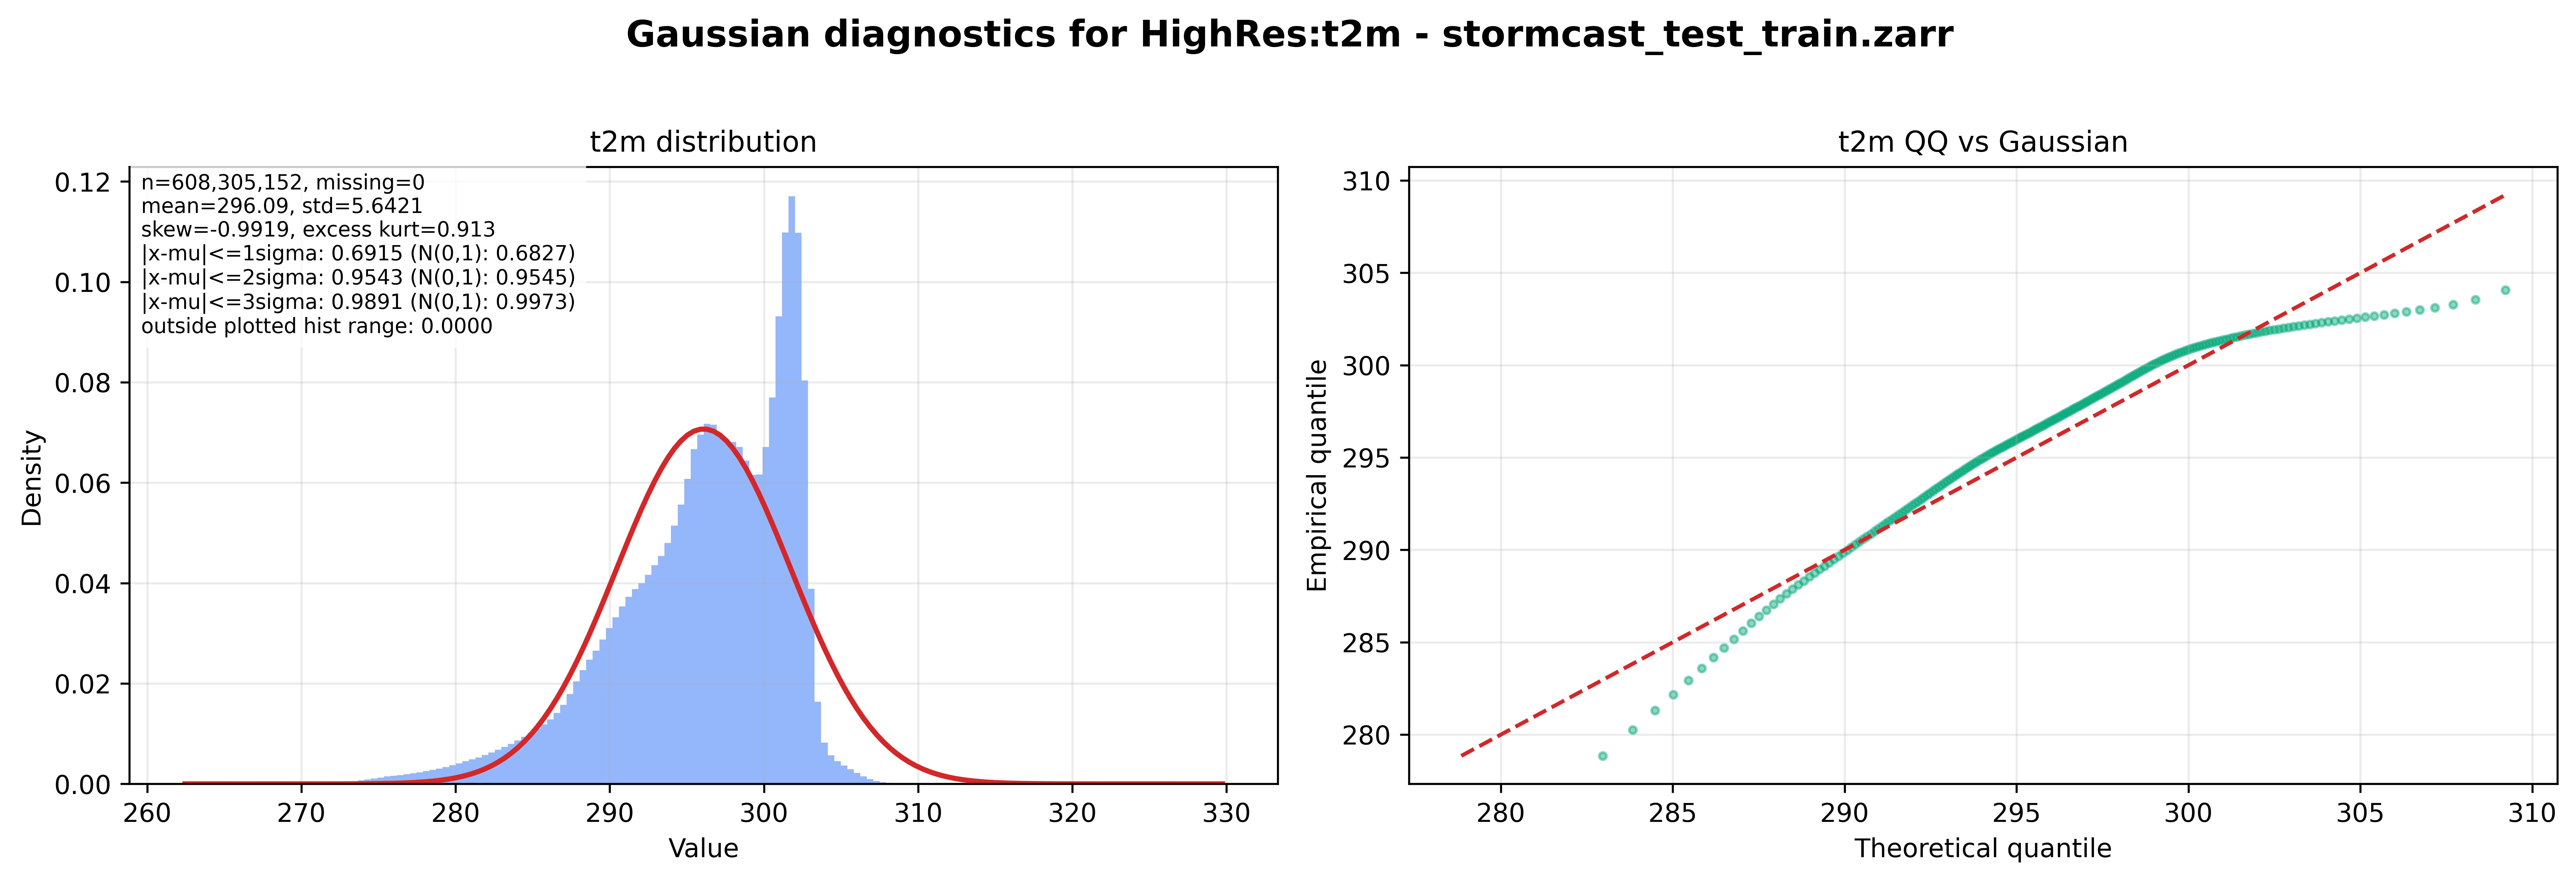
\includegraphics[width=\linewidth]{figures/highres_distributions/stormcast_test_train_HighRes_t2m_gaussian_check.png}
    \caption{\texttt{t2m} --- 2\,m temperature (K).}
  \end{subfigure}\hfill
  \begin{subfigure}[t]{0.48\linewidth}
    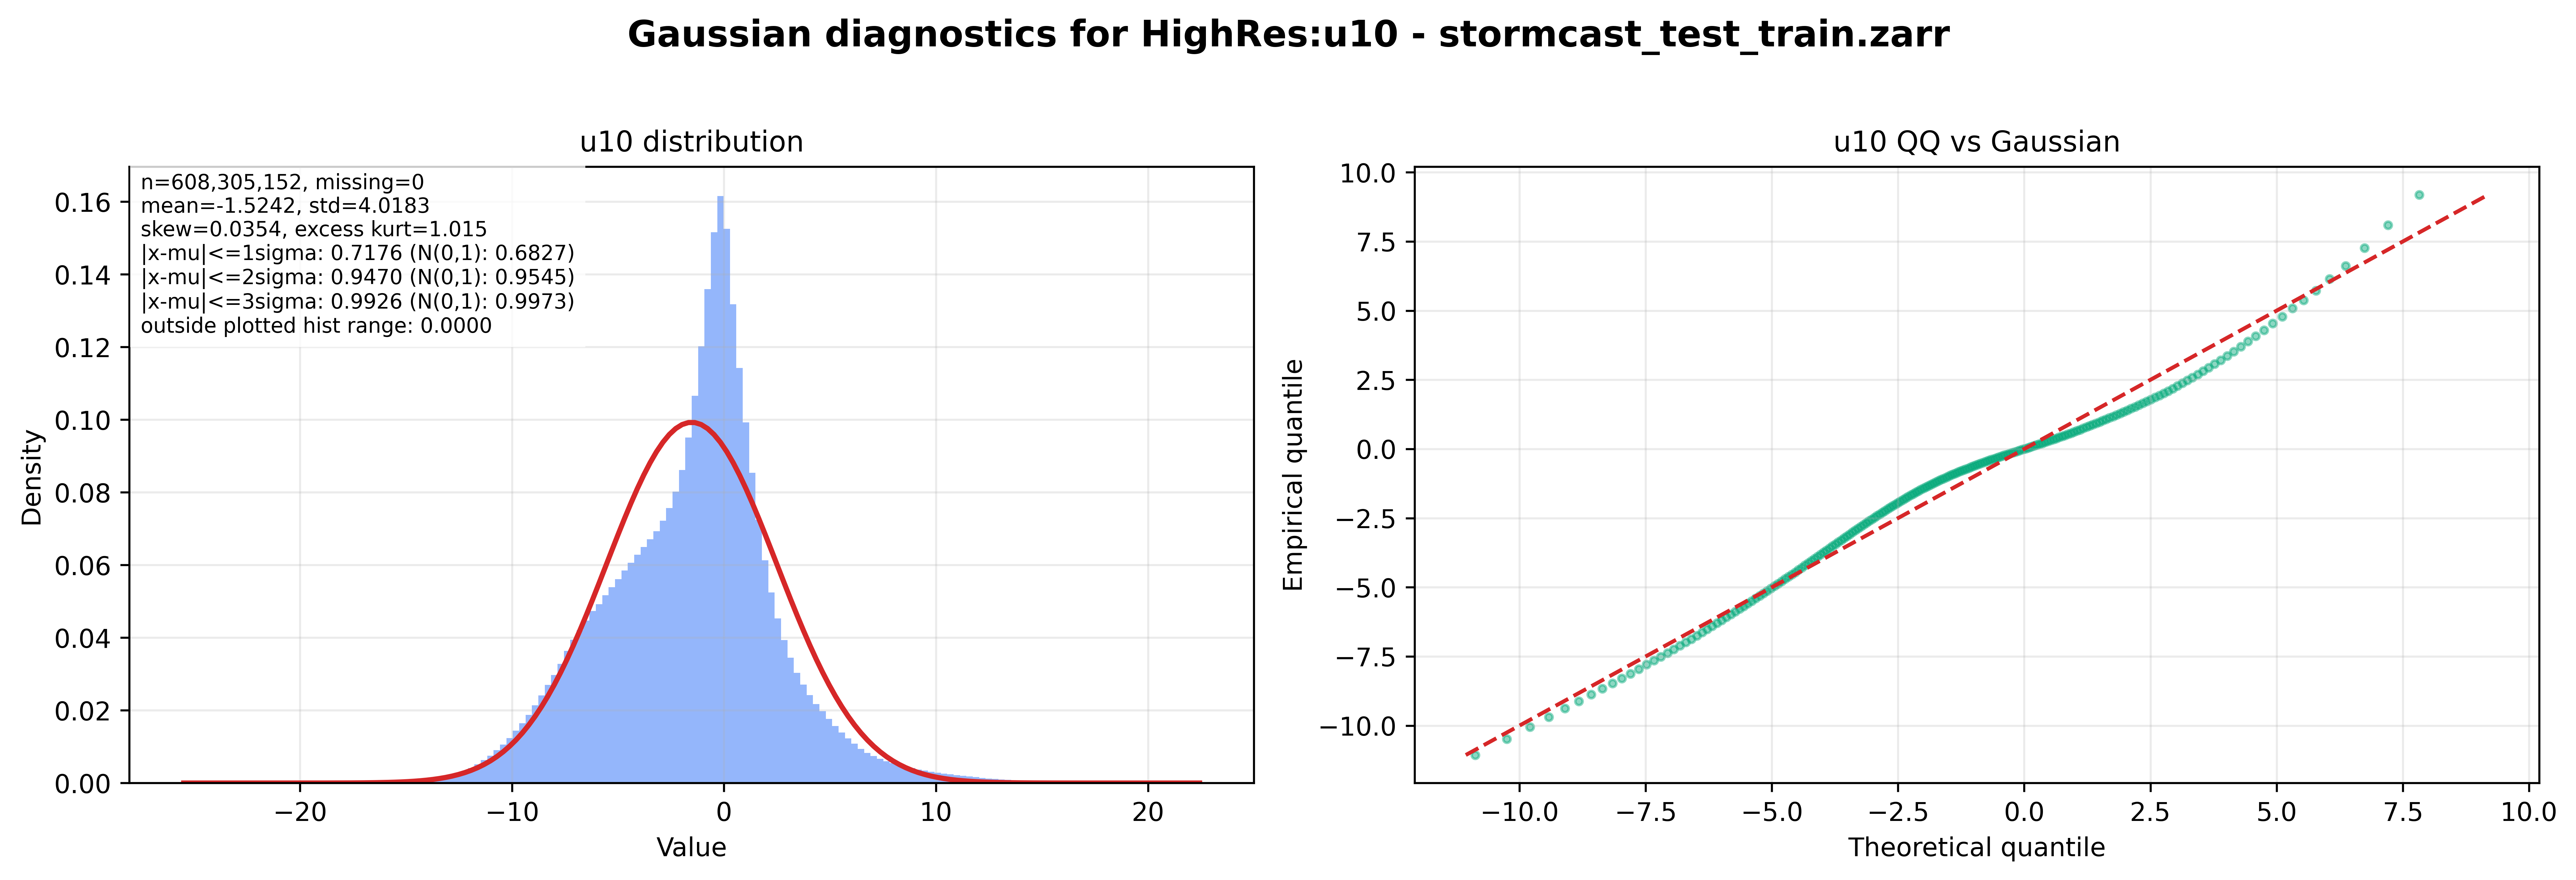
\includegraphics[width=\linewidth]{figures/highres_distributions/stormcast_test_train_HighRes_u10_gaussian_check.png}
    \caption{\texttt{u10} --- 10\,m zonal wind (m\,s$^{-1}$).}
  \end{subfigure}

  \vspace{0.5em}
  \begin{subfigure}[t]{0.48\linewidth}
    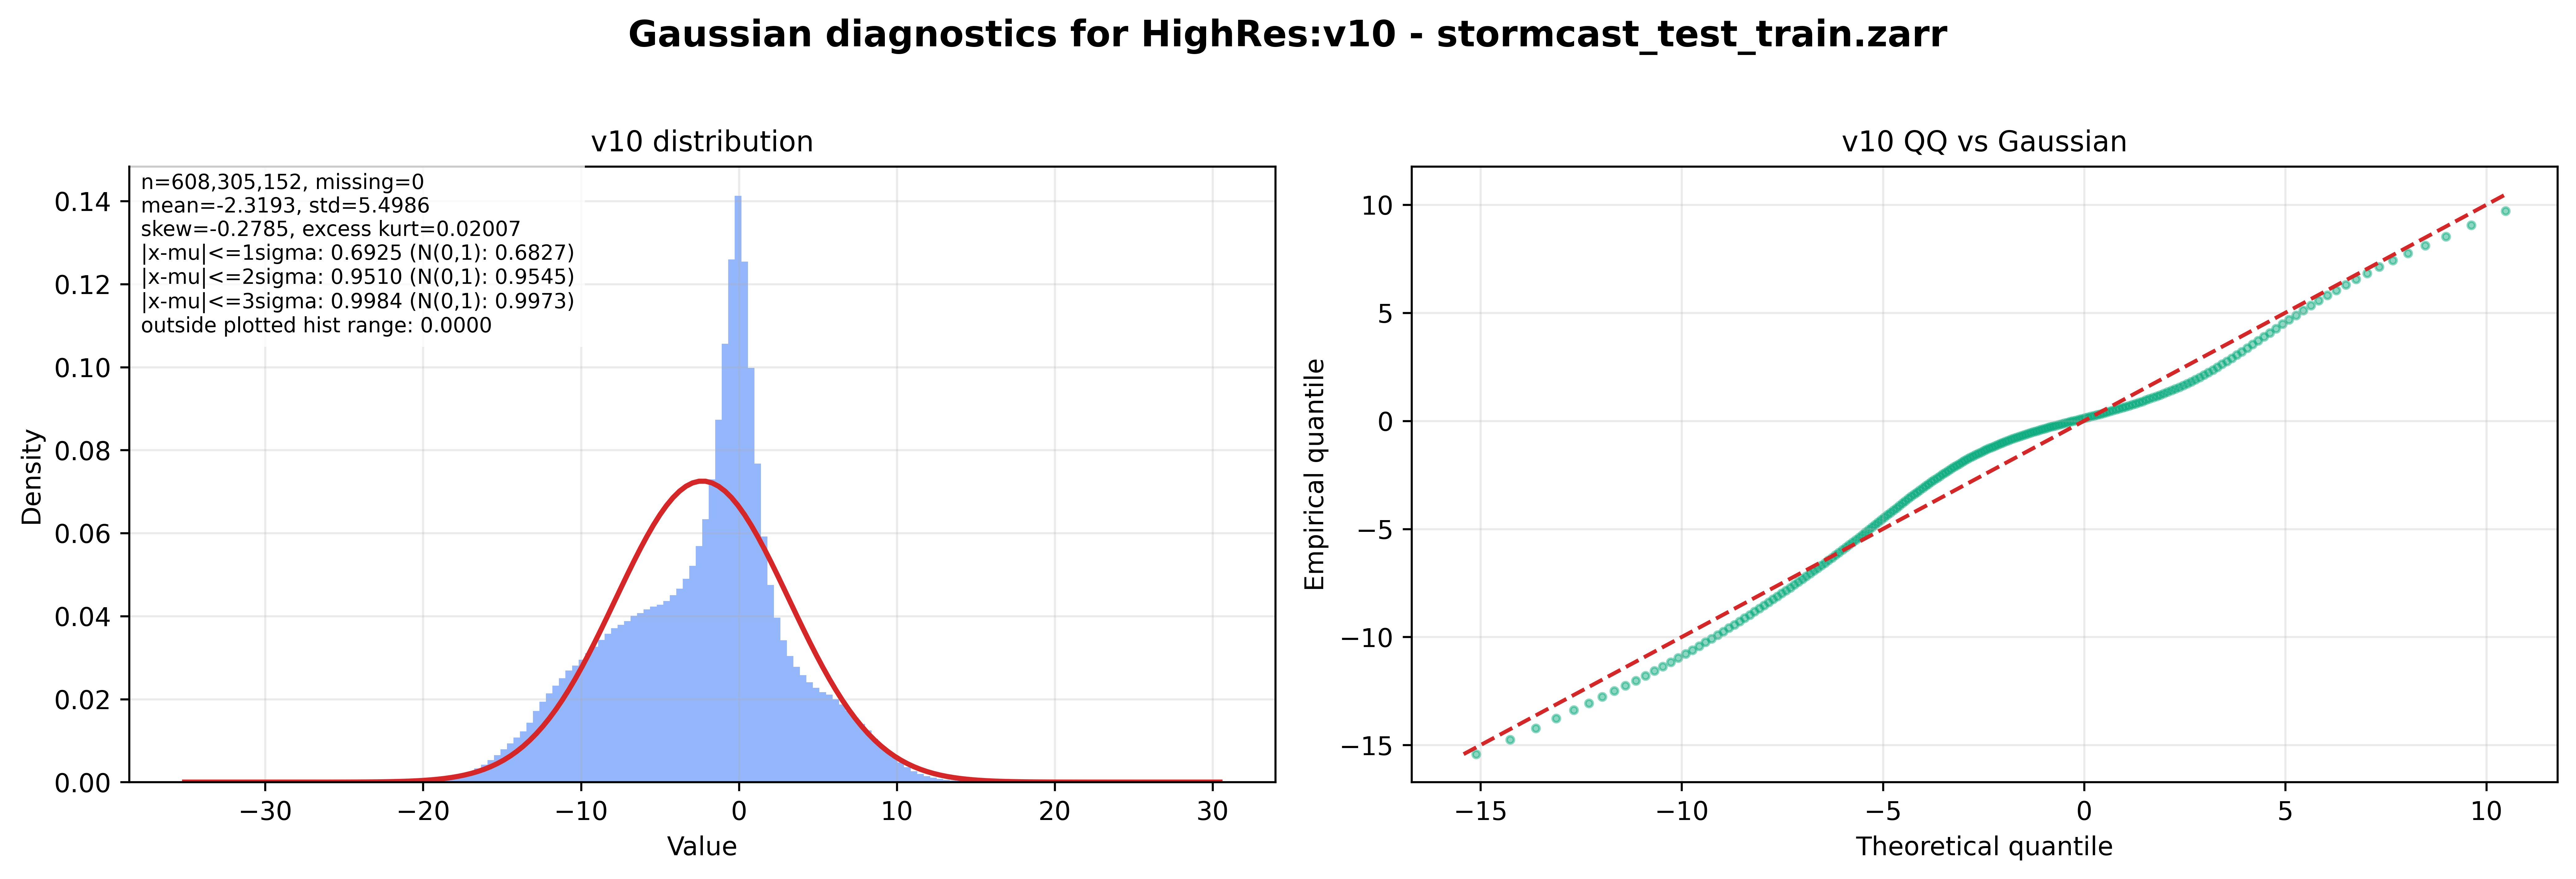
\includegraphics[width=\linewidth]{figures/highres_distributions/stormcast_test_train_HighRes_v10_gaussian_check.png}
    \caption{\texttt{v10} --- 10\,m meridional wind (m\,s$^{-1}$).}
  \end{subfigure}\hfill
  \begin{subfigure}[t]{0.48\linewidth}
    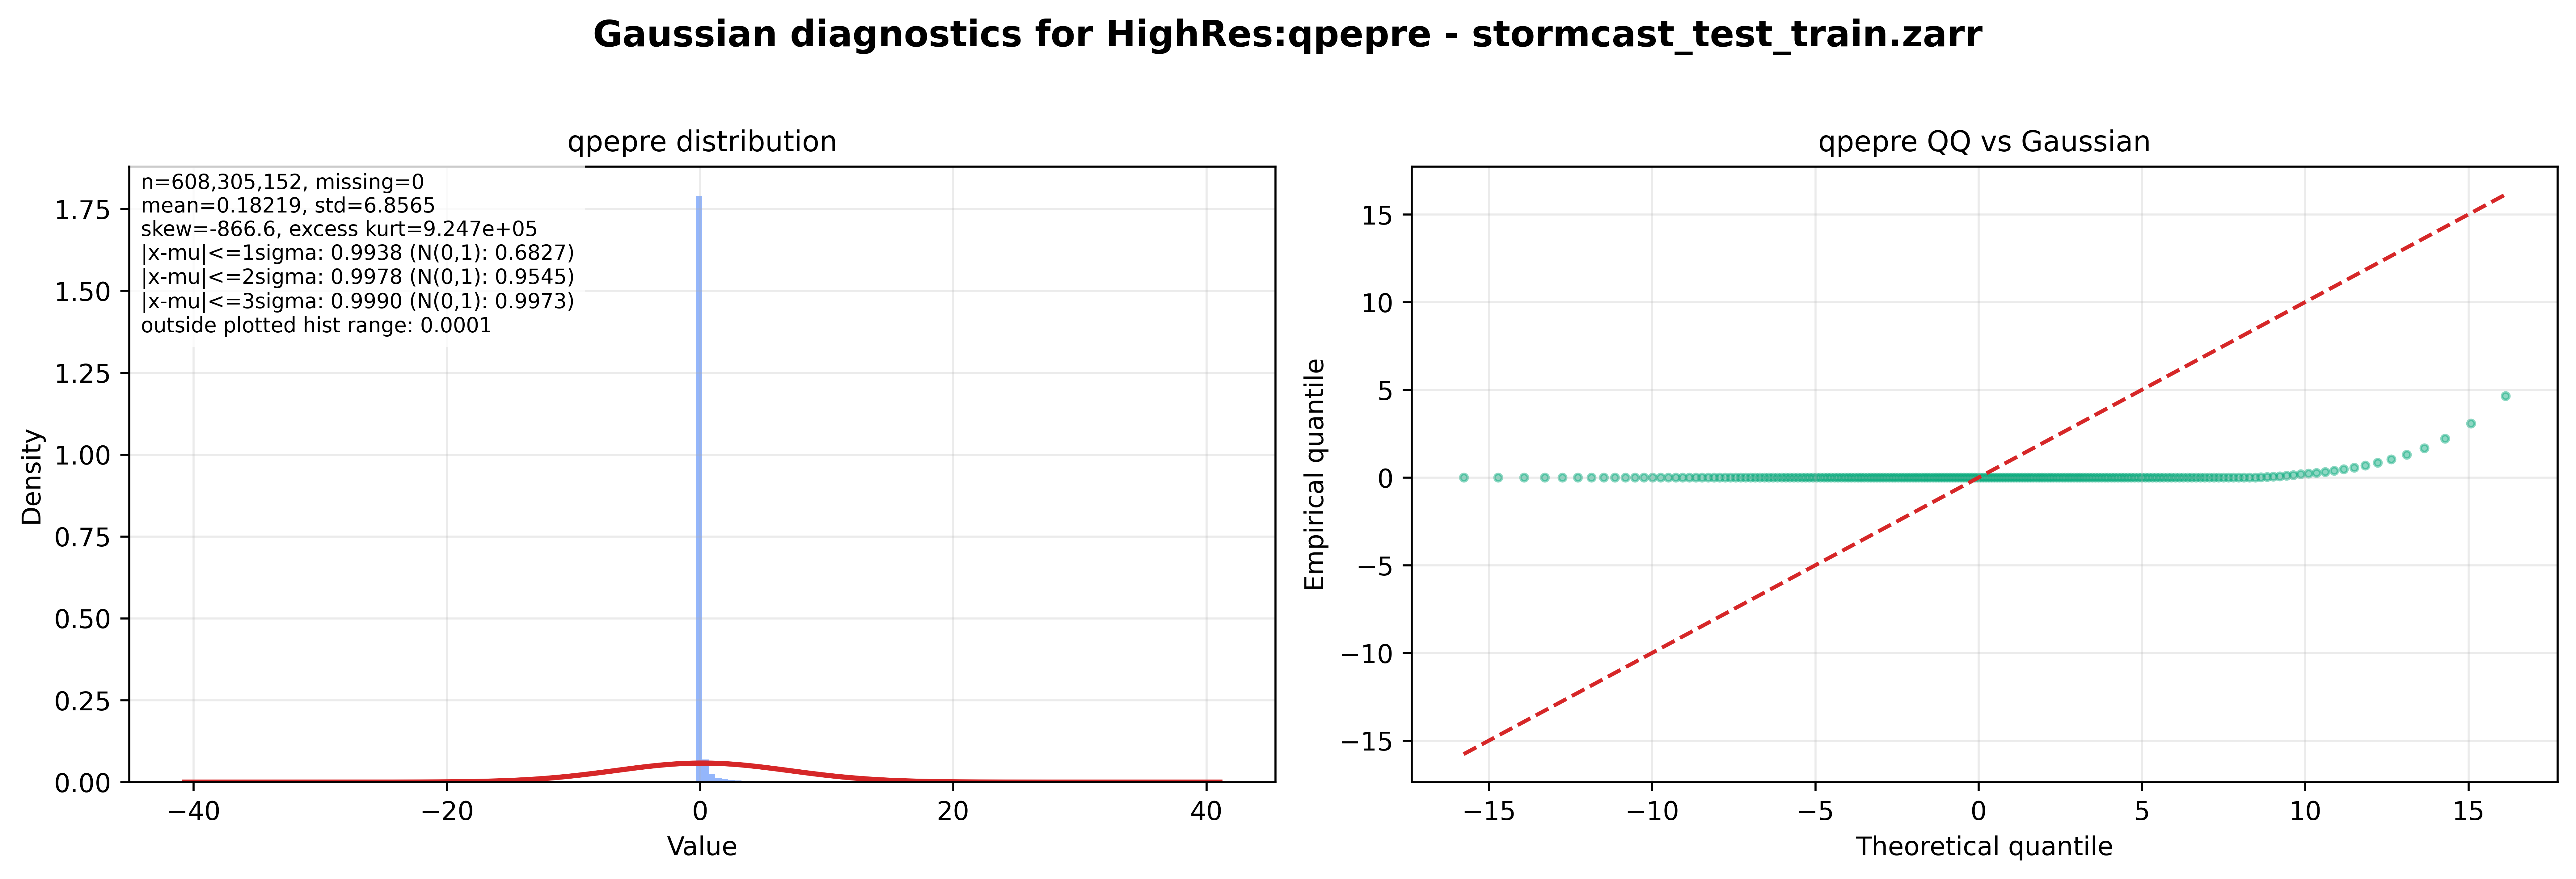
\includegraphics[width=\linewidth]{figures/highres_distributions/stormcast_test_train_HighRes_qpepre_gaussian_check.png}
    \caption{\texttt{qpepre} --- radar precipitation (mm\,h$^{-1}$).}
  \end{subfigure}
  \caption[Per-channel Gaussianity diagnostics for HighRes targets]{Per-channel distribution and Gaussian QQ plots for the four HighRes target channels over the 2.5-year training split. Left subpanels: empirical density (red) with a Gaussian fit of matched $(\mu, \sigma)$ (blue). Right subpanels: empirical quantiles against theoretical Gaussian quantiles; the red dashed line is $y=x$ for a perfect Gaussian. Generated by \texttt{data\_preprocessing/inspect\_tools/plot\_high\_res\_vars.py}.}
  \label{fig:highres-gaussian-check}
\end{figure}

\begin{table}[htbp]
  \centering
  \caption[Gaussianity statistics of HighRes target channels]{Summary statistics of the four HighRes target channels over the training split. A standard Gaussian has $\text{skew}=0$, $\text{excess kurt}=0$, and concentrates $68.3/95.5/99.7\,\%$ of its mass within $1/2/3\sigma$.}
  \label{tab:highres-gaussian-stats}
  \small
  \begin{tabular}{lrrrrrr}
    \toprule
    Channel & Mean & Std & Skewness & Excess kurt. & $\%$ in $1\sigma$ & $\%$ in $3\sigma$ \\
    \midrule
    \texttt{t2m}    & $296.09$ & $5.64$ & $-0.99$   & $0.91$      & $69.2$ & $98.9$ \\
    \texttt{u10}    & $-1.52$  & $4.02$ & $\phantom{-}0.04$    & $1.01$      & $71.8$ & $99.3$ \\
    \texttt{v10}    & $-2.32$  & $5.50$ & $-0.28$   & $0.02$      & $69.3$ & $99.8$ \\
    \texttt{qpepre} & $\phantom{-}0.18$   & $6.86$ & $-866.6$  & $9.25\times10^{5}$ & $99.4$ & $99.9$ \\
    \bottomrule
  \end{tabular}
\end{table}

The three near-surface state channels are \emph{approximately} Gaussian. \texttt{u10} is the closest: almost zero skewness, mild leptokurtosis, and a QQ plot that tracks the diagonal out to roughly $\pm 4\sigma$ before fanning into the heavy tails associated with gust events. \texttt{v10} is almost symmetric with essentially zero excess kurtosis. \texttt{t2m} is the least symmetric of the three: left-skewed (skew $= -0.99$) with a secondary mode around 280\,K corresponding to winter cold surges over northern Taiwan and the surrounding sea. For all three channels the empirical $1\sigma/2\sigma/3\sigma$ coverage agrees with the Gaussian reference to within a percentage point, which is exactly the regime for which the EDM noise schedule with $\sigma_{\text{data}}=0.5$ was designed: the teacher denoiser sees each channel as a mild deformation of a unit-variance Gaussian after normalisation, and the standard $\ell_2$ denoising loss is a reasonable fit.

\texttt{qpepre} is a different object entirely. Its marginal is dominated by an atom at zero --- the overwhelming majority of pixel-hours are dry --- with a long, very sparse tail of heavy rainfall events. The raw statistics make this quantitative: the coverage inside $\pm 1\sigma$ is $99.4\,\%$ rather than the Gaussian $68.3\,\%$, which is the signature of a near-delta distribution whose standard deviation is inflated entirely by the tail. The empirical moments reported in Table~\ref{tab:highres-gaussian-stats} (skewness $\approx -867$, excess kurtosis $\approx 10^{6}$) are formally enormous because the raw \texttt{qpepre} field uses a $-9999$ sentinel for missing observations that is only filtered at the next pipeline stage; the \emph{physical} tail above zero is still extreme (excursions beyond 100\,mm\,h$^{-1}$ occur during typhoon landfalls), but the numbers headline the practical message: the \texttt{qpepre} histogram looks nothing like a Gaussian, and the QQ plot sits on a flat shelf near zero that peels almost vertically at the upper end.

This mismatch has three consequences for diffusion-based distillation that recur throughout the rest of this thesis:
\begin{enumerate}
  \item \emph{Score matching on raw \texttt{qpepre} is ill-posed at small $\sigma$.} When the target distribution is almost a point mass at zero, the score $\nabla_x \log p_\sigma(x)$ diverges as $\sigma \to \sigma_{\min}$. The teacher partially absorbs this by learning the residual relative to the regression mean $M_t$, but the residual inherits the same atom-plus-tail shape. For this reason the consistency loss in Section~\ref{sec:method-cd} uses a Pseudo-Huber penalty rather than a pure $\ell_2$, trading a small amount of bias near zero for a bounded gradient on tail events.
  \item \emph{Pixel-wise losses undersell the tail.} Because dry pixels vastly outnumber rainy ones, an $\ell_2$ loss converges to a ``slightly wet everywhere'' solution that scores well on RMSE but destroys the convective structure we actually care about. This is the motivation for the radial log-PSD spectral regulariser applied specifically to \texttt{qpepre} in both the consistency and ADD losses, and for the precipitation-specific metrics (CSI, FSS, frequency-of-exceedance at fixed rainfall thresholds) reported in Chapter~\ref{ch:experiments}.
  \item \emph{The channel budget matters.} Because only one of the four output channels is pathological, per-channel loss weights $\beta_k$ are a natural knob: the three near-Gaussian fields can be trained with a standard denoising objective while \texttt{qpepre} receives heavier regularisation and, if needed, an $\operatorname{asinh}$ or $\log(1+x)$ transform to compress its dynamic range before the noise is added. Having only four target channels (versus the 99 of global StormCast) makes such per-channel bespoke treatment computationally trivial.
\end{enumerate}

In short, Figure~\ref{fig:highres-gaussian-check} is the quantitative justification for every ``qpepre is the hard channel'' design decision that follows: three channels live comfortably inside the Gaussian prior that diffusion assumes, and one does not.

% ==================================================
\section{Teacher Architecture Recap}
\label{sec:method-teacher}

The teacher is the two-stage StormCast model described in Section~\ref{sec:bg-regional}, with the EDM hyperparameters of Section~\ref{sec:bg-edm}.

\begin{itemize}
  \item \textbf{Regression $\Freg$.} A \texttt{StormCastUNet} taking $(X_{t-1}, S_t, I)$ as input and predicting $M_t$. The checkpoint \texttt{StormCastUNet.0.14000.mdlus} is used without modification or further training.
  \item \textbf{Diffusion $\Dteach$.} An EDMPrecond SongUNet trained to denoise the residual $R_t = X_t - M_t$ conditioned on $c_t$. The checkpoint \texttt{EDMPrecond.0.70000.mdlus} is used as the distillation teacher. EDM hyperparameters: $\sigma_{\min} = 0.002$, $\sigma_{\max} = 80$, $\sigma_{\text{data}} = 0.5$, $\rho = 7$.
\end{itemize}

Both checkpoints are loaded through the helper \texttt{get\_preconditioned\_architecture} in \texttt{stormcast/utils/nn.py}, which instantiates the network and the EDM wrapper. The conditioning bundle is assembled by \texttt{build\_network\_condition\_and\_target}, which handles the concatenation and the one-hot time-offset encoding used in the rollout.

\paragraph{Exact hyperparameter matching.} An early implementation mistake was to initialise the student with EDM hyperparameters that differed from the teacher by small amounts (for example, using $\sigma_{\text{data}} = 1.0$ instead of $0.5$). This silently broke distillation: the student's preconditioning scalings no longer aligned with the teacher's, so the loss targets were in the wrong numerical range. We therefore copy teacher hyperparameters verbatim into student configs and verify them at load time.

% ==================================================
\section{Method A: Progressive Distillation}
\label{sec:method-pd}

Our progressive-distillation pipeline follows Salimans and Ho's Algorithm 2 but operates in the EDM denoised-prediction space of $D_\theta$ rather than in the $v$-prediction space of the original paper. This matches the teacher's parameterisation and removes the need to convert between spaces at every step.

\paragraph{Phase structure.} Training proceeds through a sequence of \emph{phases}. Phase $p$ starts with a student--teacher pair sharing a schedule of $N_p$ steps; at the end of the phase, the schedule is halved to $N_{p+1} = N_p / 2$ and the student is promoted to be the new teacher. Our default phase schedule is $N_0 = 16 \to 8 \to 4 \to 2 \to 1$, producing five phases. Each phase runs for a configurable number of training steps (the default is $6 \times 10^4$).

\paragraph{Per-step loss.} Within a phase, each training step samples a mini-batch of conditioning bundles $c_t$, samples a noise level $\sigma_t$ from the EDM log-normal, forms the noised target $x_{\sigma_t} = R_t + \sigma_t \epsilon$, and then applies two teacher Heun steps to obtain $x_{\sigma_{t-2}}$. The implied one-step target $\tilde{x}$ is recovered by inverting the DDIM update
\begin{equation}
  \tilde{x} = \frac{x_{\sigma_t} - (\sigma_{t-2}/\sigma_t)\,x_{\sigma_{t-2}}}{1 - \sigma_{t-2}/\sigma_t}.
\end{equation}
The student loss is
\begin{equation}
  \mathcal{L}_{\text{PD}} = \Ebb\Bigl[w(\sigma_t)\,\|\Dnet(x_{\sigma_t}, \sigma_t; c_t) - \tilde{x}\|_{2,\beta}^2 \Bigr],
\end{equation}
where $w(\sigma_t)$ is the EDM loss weighting inherited from the teacher and $\|\cdot\|_{2,\beta}$ is the channel-weighted L2 norm defined in Section~\ref{sec:method-qpepre}.

\paragraph{Phase transitions.} At the end of each phase we (i) copy the student weights into a fresh teacher instance, (ii) halve $N$, and (iii) call \texttt{set\_num\_steps(N)} on the loss module --- a subtle but important point, because without this call the loss still computes expectations against the previous schedule and training silently fails.

\paragraph{Algorithmic summary.} Algorithm~\ref{alg:pd} gives the per-phase training loop in pseudocode form.

\begin{algorithm}[t]
\caption{Progressive-distillation phase (single halving of step count)}
\label{alg:pd}
\begin{algorithmic}[1]
\Require teacher $\Dteach$, student $\Dnet$ initialised from teacher, step count $N$, iterations $K$
\For{$k = 1, \ldots, K$}
  \State sample mini-batch $\{(X_{t-1}, S_t, X_t)\}$; form $M_t, R_t, c_t$
  \State sample noise level $\sigma_t \sim \mathrm{LogNormal}$, draw $\epsilon \sim \Nbb(0, I)$
  \State $x_{\sigma_t} \gets R_t + \sigma_t\,\epsilon$
  \State $x_{\sigma_{t-1}} \gets \mathrm{Heun}(\Dteach, x_{\sigma_t}, \sigma_t \to \sigma_{t-1}; c_t)$
  \State $x_{\sigma_{t-2}} \gets \mathrm{Heun}(\Dteach, x_{\sigma_{t-1}}, \sigma_{t-1} \to \sigma_{t-2}; c_t)$
  \State $\tilde{x} \gets \bigl(x_{\sigma_t} - (\sigma_{t-2}/\sigma_t)\,x_{\sigma_{t-2}}\bigr) / \bigl(1 - \sigma_{t-2}/\sigma_t\bigr)$
  \State $\mathcal{L} \gets w(\sigma_t)\,\|\Dnet(x_{\sigma_t}, \sigma_t; c_t) - \tilde{x}\|_{2,\beta}^2$
  \State update student parameters with Adam on $\mathcal{L}$
\EndFor
\State promote student to teacher, set $N \gets N/2$
\end{algorithmic}
\end{algorithm}

\paragraph{Implementation pointers.} The entry point is \texttt{stormcast/train\_progressive.py}; the per-phase loop lives in \texttt{stormcast/utils/trainer\_progressive.py} as \texttt{progressive\_distillation\_loop}; the loss is at \texttt{physicsnemo/experimental/metrics/diffusion/progressive\_distillation\_loss.py}; configuration is in \texttt{stormcast/config/progressive.yaml}. Inference uses \texttt{progressive\_distilled\_forward} from \texttt{stormcast/utils/nn.py}, which replaces the Heun sampler with the student's learned few-step schedule.

% ==================================================
\section{Method B: Consistency Distillation}
\label{sec:method-cd}

Consistency distillation trains $\Dnet$ to be a consistency function along teacher-generated PF-ODE trajectories, as described in Section~\ref{sec:bg-cd}. Our implementation wraps the student in a \texttt{ConsistencyPrecond} module that enforces the boundary condition $f(x, \sigma_{\min}) = x$ by the same skip-connection trick as EDM; at $\sigma = \sigma_{\min}$ the skip scaling is 1 and the output scaling is 0, so the wrapper is the identity.

\paragraph{Per-step loss.} At training iteration $k$ we read the current discretisation size $N(k)$ (see below) and sample an index $n \in \{0, \ldots, N(k) - 2\}$ uniformly. We then sample $x_0 \sim p_{\text{data}}$, form $x_{\sigma_{n+1}} = R_t + \sigma_{n+1}\epsilon$, and apply one teacher Heun step $\Phi$ to produce $x_{\sigma_n} = \Phi(x_{\sigma_{n+1}}, \sigma_{n+1} \!\to\! \sigma_n; c_t, \Dteach)$. The loss is the channel-weighted Pseudo-Huber distance
\begin{equation}
  \mathcal{L}_{\text{CD}} = \Ebb\Bigl[\rho_{c_{\text{h}}, \beta}\bigl(f_\theta(x_{\sigma_{n+1}}, \sigma_{n+1}; c_t),\; f_{\theta^-}(x_{\sigma_n}, \sigma_n; c_t)\bigr)\Bigr]
  + \lambda_{\text{spec}}\,\mathcal{L}_{\text{spec}},
\end{equation}
where $\rho_{c_{\text{h}}, \beta}(a, b) = \sum_k \beta_k\bigl(\sqrt{\|a_k - b_k\|^2 + c_{\text{h}}^2} - c_{\text{h}}\bigr)$ is the per-channel-weighted Pseudo-Huber distance, $\theta^-$ denotes the EMA copy of the student, and $\mathcal{L}_{\text{spec}}$ is the radial-PSD regulariser defined in Section~\ref{sec:method-qpepre}. We use $c_{\text{h}} = 5.4 \times 10^{-4}$, as recommended by the improved-consistency-training paper.

\paragraph{Adaptive discretisation and EMA decay.} We use the sqrt schedule
\begin{equation}
  N(k) = \left\lceil \sqrt{\frac{k}{K}\bigl(N_{\text{total}}^2 - N_0^2\bigr) + N_0^2} \right\rceil,
  \qquad
  \mu_k = \mu_0^{N_0 / N(k)},
\end{equation}
with $N_0 = 2$, $N_{\text{total}} = 150$, $\mu_0 = 0.95$, and $K$ equal to the total training iteration count. Both quantities are implemented in \texttt{stormcast/utils/ema.py} as \texttt{ema\_decay\_schedule} and \texttt{ExponentialMovingAverage}.

\paragraph{Heun teacher operator.} $\Phi$ is a single Heun step using the frozen teacher, as argued in Section~\ref{sec:bg-cd}. This matches the integrator the teacher was trained to emulate and removes an Euler-step bias term the student would otherwise absorb.

\paragraph{Inference.} One-step sampling draws $x \sim \Nbb(0, \sigma_{\max}^2 I)$ and returns $f_\theta(x, \sigma_{\max}; c_t)$. Two- and four-step sampling alternates $f_\theta$ with additive re-noising at a chosen intermediate $\sigma$. Critically, the inference weights are the EMA shadow parameters, not the online student: loading \texttt{checkpoint\_*.pt} directly yields worse samples than loading \texttt{ema\_state.pt}, and our evaluation scripts load the EMA file by default.

\paragraph{Implementation pointers.} Entry point \texttt{stormcast/train\_consistency.py}; training loop \texttt{stormcast/utils/trainer\_consistency.py}; loss \texttt{physicsnemo/experimental/metrics/diffusion/consistency\_loss.py} (\texttt{ConsistencyDistillationLoss}); configs \texttt{stormcast/config/consistency.yaml} and \texttt{stormcast/config/training/consistency.yaml}.

% ==================================================
\section{Method C: FlowCast (Conditional Flow Matching)}
\label{sec:method-flowcast}

FlowCast replaces the teacher PF-ODE with a simulation-free straight-line flow: a single network is trained from scratch to regress the target vector field $u_t = x_1 - x_0$ of Independent CFM (Section~\ref{sec:bg-flowmatching}), and sampling is a handful of Euler steps. Unlike PD and CD, FlowCast is \emph{not a distillation method} --- it does not use the EDM teacher at all --- but it is included in this thesis as a direct one-training-run alternative to few-step distilled sampling that exposes what is attributable to the teacher versus what a straight-line prior already delivers. The same StormCast residual decomposition is preserved: the deterministic regression mean $M_t$ is produced by the frozen $\Freg$, and FlowCast learns only the residual $R_t = X_t - M_t$ conditioned on a bundle $c_t$ assembled by \texttt{build\_network\_condition\_and\_target} in \texttt{stormcast/utils/nn.py}.

\paragraph{Conditioning bundle.} The conditioning channels FlowCast sees differ slightly from the EDM teacher's. The training config \texttt{stormcast/config/model/flowcast.yaml} sets
\begin{center}
\texttt{regression\_conditions: ["state", "background", "invariant"]}\\
\texttt{diffusion\_conditions: ["state", "regression", "invariant"]}
\end{center}
so the frozen regression network $\Freg$ is fed the full $(X_{t-1}, S_t, I)$ as before, but the flow-matching network itself is conditioned only on
\begin{equation}
  c_t = \mathrm{concat}\bigl(X_{t-1},\; M_t,\; I\bigr),
\end{equation}
with the low-resolution background $S_t$ deliberately omitted from the direct conditioning path. The synoptic-scale signal in $S_t$ therefore enters FlowCast only through the regression mean $M_t = \Freg(X_{t-1}, S_t, I)$. This trims the conditioning-input channel count by 24 at zero cost to the flow matching objective, because $M_t$ already summarises what the residual needs to know about $S_t$; keeping \texttt{"regression"} in the diffusion-conditions list is what keeps the FlowCast residual anchored to exactly the same $M_t$ the EDM teacher and distilled students are anchored to, which is what makes the cross-method comparison of Chapter~\ref{ch:experiments} fair.

\paragraph{Standardised-residual pipeline.} FlowCast operates on the residual in a \emph{standardised} space. The loss (\texttt{stormcast/utils/flowcast\_loss.py}) divides the raw residual by $\sigma_{\text{data}} = 0.5$ before building the flow trajectory, and the sampler (\texttt{stormcast/utils/nn.py:flowcast\_model\_forward}) multiplies the integrated state by $\sigma_{\text{data}}$ on output. Keeping $\sigma_{\text{data}}$ matched to the EDM teacher means the regression-mean anchoring statistics and the per-channel loss scaling are identical across all three methods. Concretely, with $x_1 = R_t / \sigma_{\text{data}}$ and $x_0 \sim \Nbb(0, I)$, the I-CFM interpolated state is
\begin{equation}
  x_t = (1 - t)\,x_0 + t\,x_1 + \sigma_{\text{path}}\,\eta,
  \qquad t \sim \mathcal{U}(t_\varepsilon, 1 - t_\varepsilon),\;\eta \sim \Nbb(0, I),
  \label{eq:flowcast-path}
\end{equation}
with $\sigma_{\text{path}} = 0.01$ from \citet{tong2024improving} and $t_\varepsilon = 10^{-5}$ clamping the endpoints. The small $\sigma_{\text{path}}\eta$ perturbation thickens the otherwise-Dirac conditional path $p_t(x_t \mid x_0, x_1)$ and is what separates I-CFM from the original deterministic Optimal-Transport CFM of \citet{lipman2023flow}.

\paragraph{Velocity predictor.} The student architecture is the \texttt{FlowCastPrecond} module at \texttt{stormcast/utils/flowcast\_precond.py}, instantiated through the factory call \texttt{get\_preconditioned\_architecture(name="flowcast", \ldots)} at \texttt{stormcast/utils/nn.py}. The factory wraps a SongUNet with \texttt{channel\_mult=[1, 2, 2, 2, 2]}, identical to the EDM teacher's backbone. Unlike \texttt{EDMPrecond} there are no $c_{\text{skip}}/c_{\text{in}}/c_{\text{out}}$ scalings --- the network output \emph{is} the velocity estimate:
\begin{equation}
  v_\theta(x_t, t, c_t) = \mathrm{SongUNet}\bigl(\mathrm{concat}[x_t, c_t],\; t \cdot \tau\bigr),
  \label{eq:flowcast-precond}
\end{equation}
where $\tau = 1000$ (the \texttt{time\_scale} field in \texttt{stormcast/config/model/flowcast.yaml}) rescales the flow time $t \in [0, 1]$ before it enters the SongUNet's positional-embedding layer. The SongUNet positional embedding was designed for diffusion-timestep-valued inputs with dynamic range of order $10^{2}$--$10^{3}$; feeding raw $t \in [0, 1]$ would collapse the embedding to a nearly-constant signal. $\tau = 1000$ restores enough dynamic range for the embedding to carry useful time information without changing the SongUNet itself, so no architectural changes from the teacher are needed.

\paragraph{Loss.} The training loss is the standardised-space I-CFM regression
\begin{equation}
  \mathcal{L}_{\text{FC}} = \Ebb\bigl[\,\|v_\theta(x_t, t, c_t) - (x_1 - x_0)\|_{2,\beta}^2\,\bigr] + \lambda_{\text{spec}}\,\mathcal{L}_{\text{spec}}\bigl(\hat{x}_1,\, x_1\bigr),
  \label{eq:flowcast-loss}
\end{equation}
where $\|\cdot\|_{2,\beta}$ is the per-channel-weighted L2 norm from Section~\ref{sec:method-qpepre} with $\beta = (1, 1, 1, 2)$ (the \texttt{channel\_weights} field), $\hat{x}_1 = x_t + (1 - t)\,v_\theta$ is the flow's implied clean-residual estimate at the current time, and $\mathcal{L}_{\text{spec}}$ is the radial log-PSD regulariser of Section~\ref{sec:method-qpepre} with \texttt{spectral\_channels}~$= \{\texttt{qpepre}\}$ and $\lambda_{\text{spec}} = 0.1$. Operating the spectral term on the implied-clean field $\hat{x}_1$ rather than on the raw velocity keeps the spectrum interpretable. Algorithm~\ref{alg:flowcast} summarises the per-step update.

\begin{algorithm}[t]
\caption{FlowCast training step (I-CFM on the standardised residual)}
\label{alg:flowcast}
\begin{algorithmic}[1]
\Require frozen $\Freg$, FlowCast student $v_\theta$, schedule $(\sigma_{\text{data}}, \sigma_{\text{path}}, t_\varepsilon)$, channel weights $\beta$, spectral weight $\lambda_{\text{spec}}$
\State sample mini-batch $\{(X_{t-1}, S_t, X_t)\}$; form $M_t \gets \Freg(X_{t-1}, S_t, I)$, $R_t \gets X_t - M_t$
\State build conditioning $c_t \gets \mathrm{concat}(X_{t-1}, M_t, I)$ \Comment{note: $S_t$ reaches $v_\theta$ only via $M_t$}
\State standardise: $x_1 \gets R_t / \sigma_{\text{data}}$
\State sample $x_0 \sim \Nbb(0, I)$, $t \sim \mathcal{U}(t_\varepsilon, 1 - t_\varepsilon)$, $\eta \sim \Nbb(0, I)$
\State build interpolant: $x_t \gets (1 - t)\,x_0 + t\,x_1 + \sigma_{\text{path}}\,\eta$
\State target field: $u_t \gets x_1 - x_0$
\State predict: $\hat{v} \gets v_\theta(x_t, t, c_t)$
\State pointwise: $\mathcal{L}_{\text{pw}} \gets \|\hat{v} - u_t\|_{2,\beta}^2$
\State implied clean: $\hat{x}_1 \gets x_t + (1 - t)\,\hat{v}$
\State spectral: $\mathcal{L}_{\text{spec}} \gets \frac{1}{|\mathcal{K}|}\sum_{\kappa}\bigl|\log P_{\hat{x}_1^{\text{qpepre}}}(\kappa) - \log P_{x_1^{\text{qpepre}}}(\kappa)\bigr|$
\State $\mathcal{L} \gets \mathcal{L}_{\text{pw}} + \lambda_{\text{spec}}\,\mathcal{L}_{\text{spec}}$
\State AdamW step on $\theta$; EMA update $\theta^{-} \gets 0.999\,\theta^{-} + 0.001\,\theta$
\end{algorithmic}
\end{algorithm}

\paragraph{Optimisation.} Following the FlowCast paper we use the AdamW optimiser with $\beta_{\text{Adam}} = (0.9, 0.999)$, learning rate $5 \times 10^{-4}$, and weight decay $10^{-4}$ on all parameters. The learning-rate schedule is a 4{,}000-step linear warmup (\raise.3ex\hbox{\scriptsize$\sim$}$1\%$ of the training budget) into a cosine decay to $0.01 \times 5 \times 10^{-4} = 5 \times 10^{-6}$ over the remaining steps, implemented inline in \texttt{trainer\_flowcast.py}. Gradients are globally clipped at 1.0, and per-parameter NaN gradients are sanitised with \texttt{torch.nan\_to\_num} (a safety net borrowed from the EDM trainer). Training runs for a total of 400{,}000 optimiser steps at a global batch size of 64, split across the available GPUs through PyTorch's \texttt{DistributedDataParallel}; the per-GPU micro-batch is \texttt{batch\_size\_per\_gpu = "auto"}, which the trainer resolves to $64 / W$ for $W$ workers.

\paragraph{EMA target network.} A second \texttt{FlowCastPrecond} instance is kept as an exponential-moving-average shadow of the online student, with a \emph{fixed} decay of $0.999$. The shadow is updated after every optimiser step by \texttt{ExponentialMovingAverage.update} and copied into the shadow network by \texttt{apply\_shadow} (\texttt{stormcast/utils/ema.py}). Unlike CD, where the decay $\mu_k$ is coupled to the adaptive discretisation $N(k)$, FlowCast uses a single decay throughout training because the training target (the vector field) is fixed and does not evolve with a shrinking time discretisation. The shadow weights, not the online student, are used at validation and inference time, and are saved to \texttt{ema\_state.pt} alongside each regular checkpoint. Loading the raw \texttt{checkpoint\_*.pt} instead of \texttt{ema\_state.pt} yields visibly noisier samples.

\paragraph{Sampling.} Generation integrates the learned ODE $\dot{x}_t = v_\theta(x_t, t, c_t)$ from $t = 0$ to $t = 1$ with a fixed-step solver. The implementation \texttt{flowcast\_model\_forward} in \texttt{stormcast/utils/nn.py} exposes two choices. The default is explicit Euler with $K$ steps:
\begin{equation}
  x_{t + \Delta t} = x_t + \Delta t\;v_\theta(x_t, t, c_t),
  \qquad \Delta t = 1 / K,
  \qquad x_{t=0} \sim \Nbb(0, I),
  \label{eq:flowcast-sampler}
\end{equation}
which costs $K$ NFEs. The alternative \texttt{solver="midpoint"} is a single-stage Runge--Kutta second-order scheme:
\begin{equation}
  v_{1/2} = v_\theta(x_t, t, c_t),\quad
  \tilde{x} = x_t + \tfrac{1}{2}\Delta t\,v_{1/2},\quad
  x_{t + \Delta t} = x_t + \Delta t\,v_\theta(\tilde{x}, t + \tfrac{1}{2}\Delta t, c_t),
\end{equation}
which costs $2K$ NFEs but has $O(\Delta t^{2})$ local truncation error. The sampler finishes by de-standardising: $\hat{R}_t = \sigma_{\text{data}}\,x_{t=1}$ and $\hat{X}_t = M_t + \hat{R}_t$. Validation inside the training loop uses $K = \texttt{valid\_num\_steps} = 10$ Euler steps, while the main experiments sweep $K \in \{1, 2, 4, 8, 10\}$ against the distilled students at matched NFE counts.

\paragraph{Why include FlowCast as a baseline.} Three properties of I-CFM make FlowCast the right control experiment for the distillation methods of Sections~\ref{sec:method-pd} and \ref{sec:method-cd}. First, it separates the ``few-step sampling'' question from the ``distill from a teacher'' question: any quality gap between FlowCast and the distilled students at matched NFE isolates the benefit of the teacher's signal rather than the benefit of collapsing the sampling trajectory. Second, the straight-line probability path is by construction what a one-step deterministic generator is trying to approximate, so the FlowCast $K = 1$ number is a strong reference point for the best that a single-step ODE sampler trained on the same data can do. Third, and specific to precipitation, \citet{ribeiro2025flowcast} report that I-CFM is noticeably more stable than score matching on sparse heavy-tailed fields --- a claim directly relevant to the \texttt{qpepre} channel.

\paragraph{Implementation pointers.} Entry point \texttt{stormcast/train\_flowcast.py}; training loop \texttt{stormcast/utils/trainer\_flowcast.py} (\texttt{flowcast\_training\_loop}); loss \texttt{stormcast/utils/flowcast\_loss.py} (\texttt{FlowCastLoss}); preconditioner \texttt{stormcast/utils/flowcast\_precond.py} (\texttt{FlowCastPrecond}); EMA helper \texttt{stormcast/utils/ema.py} (\texttt{ExponentialMovingAverage}); configs \texttt{stormcast/config/flowcast.yaml}, \texttt{stormcast/config/model/flowcast.yaml}, \texttt{stormcast/config/training/flowcast.yaml}; sampler \texttt{flowcast\_model\_forward} in \texttt{stormcast/utils/nn.py}. The numerical hyperparameters are tabulated in Appendix~\ref{app:hyperparams}.

% ==================================================
\section{Loss Design for the Precipitation Channel}
\label{sec:method-qpepre}

The four-channel RWRF target makes per-channel loss engineering cheap, and we use this budget to attack the hardest channel, \texttt{qpepre}, from two directions.

\paragraph{Channel-weighted Pseudo-Huber.} Let $\beta = (\beta_{\text{t2m}}, \beta_{\text{u10}}, \beta_{\text{v10}}, \beta_{\text{qpepre}})$ be a vector of non-negative per-channel weights. The weighted L2 and Pseudo-Huber norms are
\begin{equation}
  \|a\|_{2,\beta}^2 = \sum_{k=1}^{4} \beta_k\,\|a_k\|^2,
  \qquad
  \rho_{c_{\text{h}}, \beta}(a, b) = \sum_{k=1}^{4} \beta_k\bigl(\sqrt{\|a_k - b_k\|^2 + c_{\text{h}}^2} - c_{\text{h}}\bigr),
\end{equation}
where the sum runs over the four output channels and the norm inside each term is the ordinary spatial L2. The default configuration uses $\beta = (1, 1, 1, w_{\text{pr}})$ with $w_{\text{pr}} \in \{2, 4\}$ to compensate for the precipitation channel's smaller effective signal under the Pseudo-Huber loss. These weights are exposed as \texttt{channel\_weights} in the consistency-loss config.

\paragraph{Radial log-PSD regulariser.} Because RMSE-like losses reward smooth, low-amplitude precipitation outputs, we add a spectral-matching regulariser that penalises the L1 distance between the radial log-PSD of the predicted and target \texttt{qpepre} fields:
\begin{equation}
  \mathcal{L}_{\text{spec}} = \frac{1}{|\mathcal{K}|}\sum_{\kappa \in \mathcal{K}} \bigl|\log P_{\text{pred}}(\kappa) - \log P_{\text{target}}(\kappa)\bigr|,
\end{equation}
where $P(\kappa)$ is the radially averaged 2D power spectral density at wavenumber $\kappa$ and $\mathcal{K}$ is the set of non-zero radial wavenumbers on the $224 \times 128$ grid. The regulariser is active only on channels listed in \texttt{spectral\_channels} and weighted by \texttt{spectral\_weight} $= \lambda_{\text{spec}}$. By default we apply it to \texttt{qpepre} only.

\paragraph{Monitoring for mode collapse.} Even with the above terms, sparse heavy-tailed precipitation is an invitation to mode collapse: the model can minimise both MSE and Pseudo-Huber by producing a slightly-wet constant field. During training we therefore log the wet-pixel fraction at thresholds $\{0.1, 1.0, 5.0\}$\,\si{\milli\metre\per\hour} and the 95th and 99th percentiles of the output distribution, and compare them to the same quantities on the training batch. A large divergence is a collapse warning.

% ==================================================
\section{Training Infrastructure}
\label{sec:method-infra}

All runs use PyTorch with \texttt{torchrun --standalone --nnodes=1 --nproc\_per\_node=N} for multi-GPU training. Configuration is managed with Hydra; experiment overrides are passed on the command line as \texttt{key=value} pairs. Checkpoints are written every $M$ iterations (default $M = 1000$) under
\begin{center}
\texttt{StormCast\_\{method\}/\{experiment\}/0/checkpoints\{\_method\}/checkpoint\_*.pt}
\end{center}
together with CSV loss logs and, every $V$ iterations, validation heatmap and power-spectrum images for the four output channels. Auto-resume is implemented by \texttt{\_detect\_resume\_state} in the progressive trainer and by a \texttt{checkpoint\_latest.pt} convention in the consistency trainer. A run can therefore be restarted with the same command line and will pick up from the last written checkpoint.
